
\subsection*{Composition of Functions}
There are several ways to combine two existing functions to create a new function.  For example, in calculus, we learned how to form the product and quotient of two functions and then how to use the product rule to determine the derivative of a product of two functions and the quotient rule to determine the derivative of the quotient of two functions.

The chain rule in calculus was used to determine the derivative of the composition of two functions, and in this section,  we will focus only on the composition of two functions.  We will then consider some results about the compositions of injections and surjections.

The basic idea of function composition is that when possible, the output of a function  $f$  is used as the input of a function  $g$.  This can be referred to as ``$f$  followed by  $g$'' and is called the composition of  $f$  and  $g$. In previous mathematics courses, we used this idea to determine a formula for the composition of two real functions.

For example, if
\[
f( x ) = 3x^2  + 2 \quad \text{and} \quad g( x ) = \sin x, 
\]
then we can compute  $g( f( x ) )$  as follows:
\[
\begin{aligned}
  \hfill g( {f( x )} ) &= g \! \left( {3x^2  + 2} \right) \\
                       &= \sin \! \left( {3x^2  + 2} \right). \\ 
\end{aligned} 
\]
In this case,  $f( x )$, the output of the function  $f$, was used as the input for the function  $g$.  We now give the formal definition of the composition of two functions.  
\begin{defbox}{functioncomposition}{Let  $A$, $B$, and  $C$  be nonempty sets, and let  
$f\x A \to B$  and  $g\x B \to C$  be functions.  The \textbf{composition of}
\index{composition of functions}%
\index{function!composition}%
  $\boldsymbol{f}$ \textbf{and} $\boldsymbol{g}$  is the function  $g \circ f\x A \to C$  defined by
\label{sym:composition}
\[
( {g \circ f} )( x ) = g\left( {f( x )} \right)
\]
for all  $x \in A$.  We often refer to the function  $g \circ f$ as a \textbf{composite function}.
\index{function!composite}%
\index{composite function}%
}
\end{defbox}
It is helpful to think of the composite function  $g \circ f$
 as  ``$\boldsymbol{f}$  \textbf{followed by}  $\boldsymbol{g}$.''  We then refer to  $f$  as the \textbf{inner function}
\index{inner function}%
\index{composition of functions!inner function}%
 and  $g$  as the \textbf{outer function}.
\index{outer function}%
\index{composition of functions!outer function}%


%\begin{prog}[\textbf{Order of the Composition of Two Functions}] \label{pr:composeorder} \hfill \\
%Let  $h\x \mathbb{R} \to \mathbb{R}$ be defined by  $h( x ) = 3x + 2$ and  $g\x \mathbb{R} \to \mathbb{R}$ be defined by  $g( x ) = x^3 $.  Determine formulas for the composite functions  $g \circ h$  and  $h \circ g$.  What does this tell you about the operation of composition of functions?
%\end{prog}
%\hbreak

\subsection*{Composition and Arrow Diagrams} 
The concept of the composition of two functions can be illustrated with arrow diagrams when the domain and codomain of the functions are small, finite sets.  Although the term ``composition'' was not used then, this was done in \typeu Activity~\ref*{PA:compositionintro}, and another example is given here.

Let  $A = \left\{ {a, b, c, d} \right\}$, $B = \left\{ {p, q, r} \right\}$, and  
$C = \left\{ {s, t, u, v} \right\}$.  The arrow diagram in Figure~\ref{fig:arrow64-1} shows two functions:  
$f\x A \to B$  and  $g\x B \to C$.
\begin{figure}[h]
\begin{center}
\scalebox{0.95}{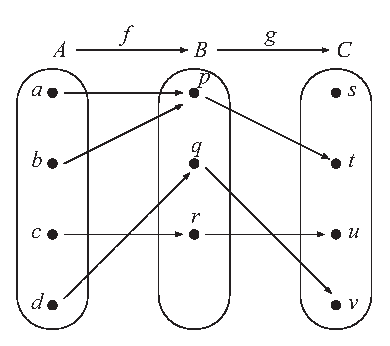
\includegraphics{figps-sec641.eps}} 
\caption{Arrow Diagram for Two Functions} \label{fig:arrow64-1}
\end{center}
\end{figure}

If we follow the arrows from the set  $A$  to the set  $C$, we will use the outputs of  $f$  as inputs of  $g$, and get the arrow diagram from  $A$  to  $C$ shown in Figure~\ref{fig:arrow64-2}.  This diagram represents the composition of  $f$  followed by  $g$.
\begin{figure}[h]
\begin{center}
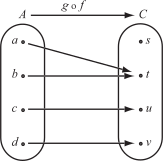
\includegraphics{figps-sec642.eps} 
\caption{Arrow Diagram for $g \circ f\x  A \to C$} \label{fig:arrow64-2}
\end{center}
\end{figure}
%
%


%\pagebreak
\begin{prog}[\textbf{The Composition of Two Functions}] \label{pr:compose} \hfill \\
Let $A = \{ a, b, c, d \}$ and $B = \{ 1, 2, 3 \}$.  Define the functions $f$ and $g$ as follows:
\begin{list}{}
\item $f \x A \to B$ defined by $f(a) = 2$, $f(b) = 3$, $f(c) = 1$, and $f(d) = 2$.
\item $g \x B \to B$ defined by $g(1) = 3$, $g(2) = 1$, and $g(3) = 2$.
\end{list}

\newpar
Create arrow diagrams for the functions $f$, $g$, $g \circ f$, and $g \circ g$.
\end{prog}
\hbreak



\endinput
